\documentclass[runningheads]{AIIT}
%\usepackage[utf8]{inputenc}
%\usepackage[russian]{babel}
\usepackage{graphicx}
\usepackage{hyperref}

%---------- BEGIN May be removed ------------------
% \usepackage[usenames,dvipsnames,svgnames,table]{xcolor}
% \definecolor{rclr}{rgb}{0.5,0.1,0.1}
% \definecolor{eclr}{rgb}{0,0.5,0.5}
% \colorlet{acolor}{blue}
% \colorlet{rcolor}{red}
% \definecolor{ncolor}{rgb}{0.5,0.5,0.1}
% \newcommand{\aaa}[2][acolor]{\noindent\textcolor{eclr}%
% {+\ [}\textcolor{#1}{#2}\textcolor{eclr}{]}}
% \newcommand{\rrr}[2][rcolor]{\noindent%
% \textcolor{eclr}{-\ [}\textcolor{#1}{#2}\textcolor{eclr}{]}}
% \newcommand{\nnn}[2][rcolor]{\noindent%
% \textcolor{eclr}{}\textcolor{#1}{#2}\textcolor{eclr}{}}
%---------- END May be removed ------------------

\hypersetup{
    bookmarks=true,         % show bookmarks bar?
    unicode=true,           % non-Latin characters in Acrobat’s bookmarks
    pdftoolbar=true,        % show Acrobat’s toolbar?
    pdfmenubar=true,        % show Acrobat’s menu?
    pdffitwindow=false,     % window fit to page when opened
    pdfstartview={FitH},    % fits the width of the page to the window
    pdftitle={Expert System for Structural Analysis\\ of Electrocardiogramms},    % title
    pdfauthor={Kristina Krasovitskaya, Evgeny Cherkashin, Sergey Gorunchik},     % author
    pdfsubject={Electro cardio signal processing and recognition},   % subject of the document
    pdfcreator={EMACS-24.5:AuCTeX-0.89},   % creator of the document
    pdfproducer={PdfLaTeX}, % producer of the document
    pdfkeywords={electrocardiogram} {ECG} {expert system} {ECG recognition}
      {electrocardiosignal} {time series recognition} {image processing}
      {continuous wavelet transformation}, % list of keywords
    pdfnewwindow=true,      % links in new window
    colorlinks=true,       % false: boxed links; true: colored links
    linkcolor=black,          % color of internal links (black)
    citecolor=black,        % color of links to bibliography
    filecolor=black,      % color of file links
    urlcolor=black           % color of external links
}


%% Necessary definitions for the running heads
\def\journalissue{International Conference on Applied Internet and Information Technologies, 2016}
\def\paperidnum{DOI: N/A}
\setcounter{page}{1}

\title{Expert System for Structural Analysis\\ of Electrocardiograms}

%% Use this if the title is too long for the running heads
\titlerunning{Expert System for ECS}

\author{Kristina Krasovitskaya\inst{1} \and Evgeny Cherkashin\inst{2} \and Sergey Gorunchik\inst{3}}

%% Use this the list of authors is too long for the running heads
%\authorrunning{First Author et al.}

\institute{Irkutsk National Research Technical University,\\
Lermontov str. 83, Irkutsk, 664074, Russian Federation\\
  \email{kristina.kras1993@gmail.com}
  \and
Matrosov Institute for System Dynamics and Control Theory of\\
Siberian Branch of Russian Academy of Sciences,\\
Lermontov str. 134, Irkutsk, 664033, Russian Federation\\
  \email{eugeneai@icc.ru}
  \and
  Specialized Tuberculosis Hospital in Rostov region,\\
Orskaya str. 24, Rostov-on-Don, 344000, Russian Federation\\
  \email{sergeygreen@mail.ru}}
\begin{document}
%\selectlanguage{}
\maketitle

\begin{abstract}
The paper deals with process of a cardiological expert system development. A definition of a electrocardiogram is presented. Problems of ECG characteristics determination such as ECG data digitizing is considered. A problem of QRS complex recognition and P and T waves parameters measurement is discussed. A general outline of analysis technique for ECG using wavelet transformation are proposed.

\vspace{6pt}\textbf{Keywords:} electrocardiogram, ECG, expert system, ECG recognition, electrocardiosignal, time series recognition, image processing, continuous wavelet transformation.
\end{abstract}

\section{Introduction}

Medical images are popular objects of automatic analysis.  An image of an electrocardiogram (ECG) contains time series of a cardiosignals, which are processed synchronously.  Manual static analysis is always a multistage process.  The signal processing software delivered with a cardiological diagnosis is intended for experienced functional diagnostician and rigidly bound to the appliance model, resulting to impossibility to make a comparative analysis of ECGs of the same patient data obtained in different medical centers and time moments.  This, in turn, implies additional examination to be carried on the patient to obtain the time series in a required file and data format, increasing the cost of the patient residence in the diagnostic center.  Also, Russia has regions where the specialized professional cardiological treatment is not possible, this can lead to fatal complications due to time delays.

In order to improve the quality and accessibility of medical cardiology provision for the population, Ministry of Health of Russian Federation started to elaborate of a law project aimed at a legal basis construction of IT infrastructure for public health protection.  The infrastructure will be based on remote interaction of medical professionals and patients.  At present the interaction (such as remote consultations) is out of professional moderation and provided via forums, specialized internet sites and Skype.  The cardiological data is supplied as attached photographic as scanned images.  The final conclusions made in the environment are of question.

The automatic processing and analysis of the ECG will reduce human factor impact on the final conclusion since automatic processing results are not affected by the degree of fatigue, observation time, and body physical condition of the physician.  Moreover the results produced by human expert are usually intuitive, expressed in quality statements, and the reasoning process can be hardly represented as explicit elementary stages (as an algorithm).  For example, expert estimates the width of PQ interval to be shorter as compared to one described in the literature, in addition, the subjective estimation varies among specialists \cite{rangaraj}. Computer processing and analysis is significantly formalized and operates by qualitative values.

The computational ECG processing has already more than fifteen years.  But it seems that there are no industry standards of data representation and processing pipelines of the EGC images as well as complete set of methods, data formats, IT tools and techniques for implementation of each stage of the pipeline.  The ECG image processing problem is classified as artificial intelligence recognition task with the lack and data distortion.

Among the existing ECG processing software made in Russian Federation we emphasize system ``Valenta'' as a popular software tool for ECG data analysis obtained from its instrument.  The program does not allow processing data from other sources such as scanned tape images and time series obtained from other appliances.  Monitor control systems, e.g., arrhythmia monitor system ``Argus'', require special equipment.  Professor MD V.~M.~Uspensky suggested new diagnostic method that allows expert to diagnose a wide range of deceases of internal organs by describing a ECG.  The method does not allow one to diagnose an essential set of hearth deceases causing arrhythmia that has 8\% of all the cases in last three years.  The analytic systems do not support importing raster graphics of scanned images of ECG printed on a paper --- still the most popular media.  Digitizing such sources and extraction of time series allow us to organize automated diagnostic environments on the base of electronic medical records.

In this investigation we develop an IT technique and software, which will process and analyze ECG raster images obtained in cardiologist's offices, medical organizations and from medical histories.  The aim of the investigation is to develop software allowing cardiologists to watch the dynamics as an ECG evolution in time.  To achieve so we need to digitize ECG time series, filter parasite distortions (low and high frequency), straighten the signal base, and measure signal relative entity sizes in \% to the reference ones.  Another problem is automatic interpretation of an ECG as a result of signal form analysis.  The automatic analysis as a pedantic and formal procedure will rise the probability to mention, e.g., atrial fibrillation, and lower human factor in decision making.


\section{Structire of ECG}
\label{sec:structire-ecg}

\emph{Electrocardiogram} (ECG) is a graphical representation (a time series records) of impulse conduction on the nodes and bundles of the cardiac conduction system of heart.  ECG is recorded as a number of \emph{electrical entities} (\emph{pikes} made of rising and drooping, and \emph{horizontal segments}) \cite{wikipedia}.  Pike entities are denoted by letters P, Q, R, S and T, whereas horizontal segments are denoted by PR segment and ST segment.

Each ECG analysis is started from verification of the registration process.  The registration of hearth electric field potential, named as \emph{lead}, is measured between two placements of the chest surface.  The standard ECG consists of twelve leads (vectors): three 2-pole (3 standard leads), three 1-pole reinforced limb leads, six 1-pole chest leads.

\begin{figure}[htb]
  \centering
    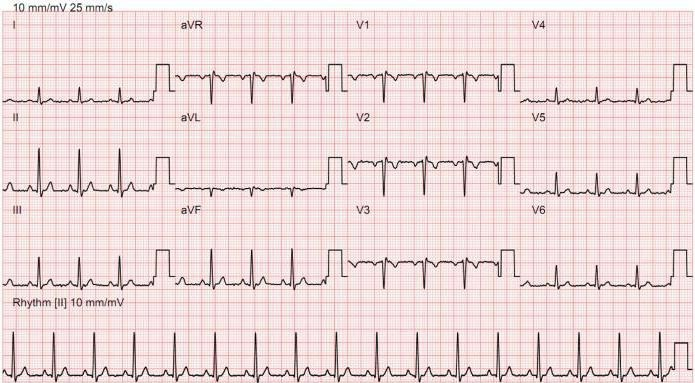
\includegraphics[width=0.5\linewidth]{images/Stand_ECG.jpg}
  \caption{Standard twelve-lead ECG}
  \label{fig:leads-ex}
\end{figure}

\section{Image processing}
\label{sec:image-processing}

\subsection{Recognition of lead time series}
\label{sec:digit-recogn}

% Time series digitizing
The first stage of the ECG image processing is a recognition of the time series if the leads.  The source image scan consists of tracing paper background with square grid and lines of time series.  Time series include a reference pulse at the beginning (Fig.~\ref{fig:leads-ex}).  The processing of the image can be done with various techniques.  We started directly from the application of edge tracing algorithms and obtained the results like ones depicted in Fig.~\ref{fig:sobel-ex}.

\begin{figure}[htb]
  \centering
    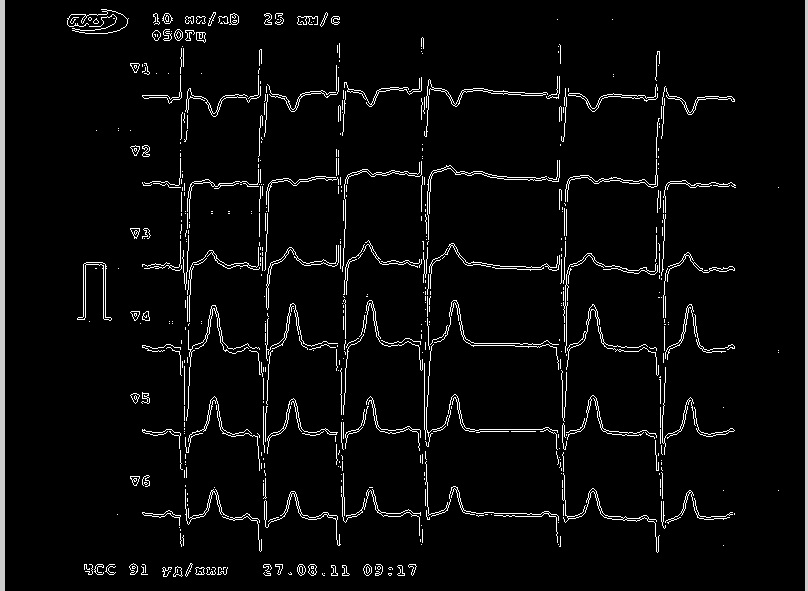
\includegraphics[width=0.5\linewidth] {images/Sobel.jpg}
  \caption{Sobel filter processing (inverted)}
  \label{fig:sobel-ex}
\end{figure}

As the image consists of the combination of the background and signal time series, we decided to filter out the background \cite{gonseles,1}.  The following schema implements the filtering.
\begin{enumerate}
\item A color channel of the background hue is extracted from the source image.
\item A red image copy is blurred with Gaussian filter in the red channel.
\item The digital image of the lead time series is obtained using the following formula:
  $s(n)=f(n)+\sigma e(n)$, where $f(n)$ is the signal, $\sigma$ is the
  noise level, $e(n)$ is the Gaussian white noise, and $s(n)$ is the original
  signal.  The threshold transformation is applied to the image as well.
\item The signal recording is restored in a cyclic processing of the columns of the obtained pixel array of the image.
\end{enumerate}
The algorithm did not produce results on all the test given.  Ten out of 156 ECGs did not completely analyzed due to threshold transformation function faults.  The function parameters were adjusted by means of a machine learning technique.  Hue and brightness characteristics of each column of the image were used as attributes of input train set.

\begin{figure}[htb]
  \centering
    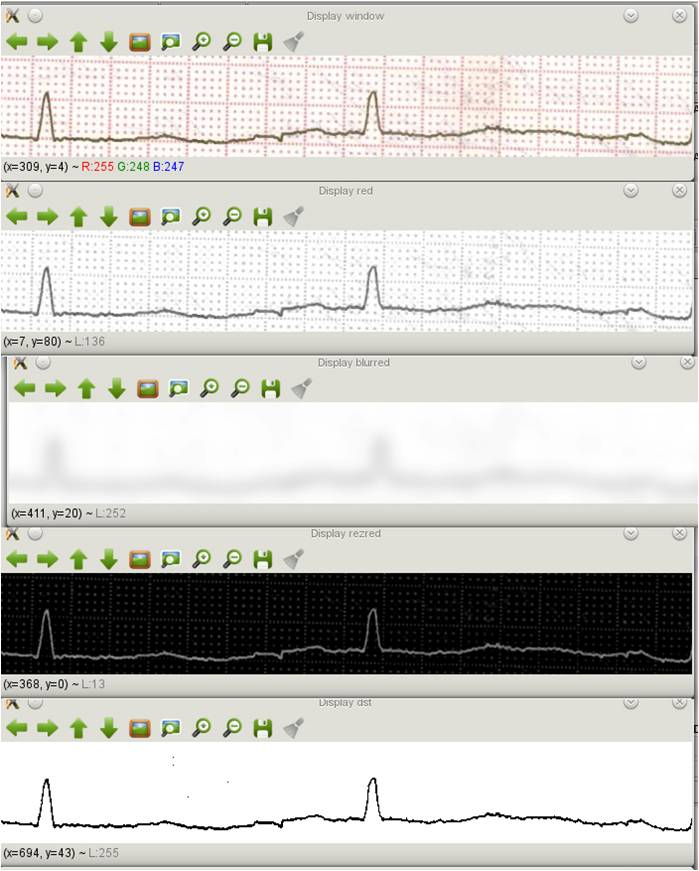
\includegraphics[width=0.5\linewidth] {images/Algorithm.jpg}
  \caption{Algorithm stages of time series recognition}
  \label{fig:leads-ex}
\end{figure}

\subsection{Time series post processing}
\label{sec:cleaning-artefacts}

The original ECG image in a general case contains signal distortions such as baseline drift and proximity effect to energy supply network.  A similar low frequency distortion could also be introduces by time series recognition algorithms.  The baseline drift arises due to patient's strong movement, electrode polarization, appliance measurement error, and poor electrode contact to patient's skin.  We used discrete Butterworth filter in the removal procedure of the low frequency distortions
$$
|H(k)|^2=\frac{1}{1+(k/k_c)^{2N}},
$$
where $H$ is frequency response of the analog filter, $k_c$ is a cutoff frequency (rad/s), $k$ is the analog frequency in radiant.  The energy supply network has usually 50 or 60 Hertz frequency, and its distortion is suppressed with band-stop and comb filters.

In the case when many copies of ECG is accessible, one can take advantage of synchronous and ensemble averaging techniques.  The noise is a stationary stochastic process, and the ECG signal itself is (quasi-) periodical or cyclically-stationary.  Sliding mean filer in time space is applicable to a statistically stationary low frequency signals.  This technique provides filtering capabilities in real time mode.

If the real time mode is not required we use filtering in the frequency space.  If a power spectral density and autocorrelation function parameters are known, one can make use of optimal Wiener filter.  If the noise is not correlated to the signal or the distortion has nonstationary (or even stochastic) properties and there are no additional data, but we have a record from a secondary source, then adaptive filtering is used.

\section{ECG entities recognition}
\label{sec:ecg-etit-recogn}

\subsection{QRS complex detection}
\label{sec:qrs-compl-detect}

The QRS complex detection is usually based on locating R pike with the following removal of the whole QRS complex from the ECG time series.  The R location can be obtained by means of various methods, e.g., based on the derivative \cite{Ahlstrom-Tomhins}, sliding mean filer, weighted and squared operators of the first derivative \cite{Murthy-Rangaraj}, detection algorithm of Pan-Tompkins \cite{Pan-Tomhins}.  For PQRST complex detection, there are discrete wavelet transformation based algorithms \cite{Daqrouq,Dubrovin}, and duration transformation \cite{Gritzali}.

In this project we used discrete wavelet transformation method as it can determine pikes in the signals with base line drift distortion.  The previously recognized time series are loaded from a file, and 4th degree wavelet decomposition is computed over the loaded data (Fig.~\ref{fig:decomp}), the source signal is decomposed with Daubechies wavelet.

\begin{figure}[htb]
  \centering
    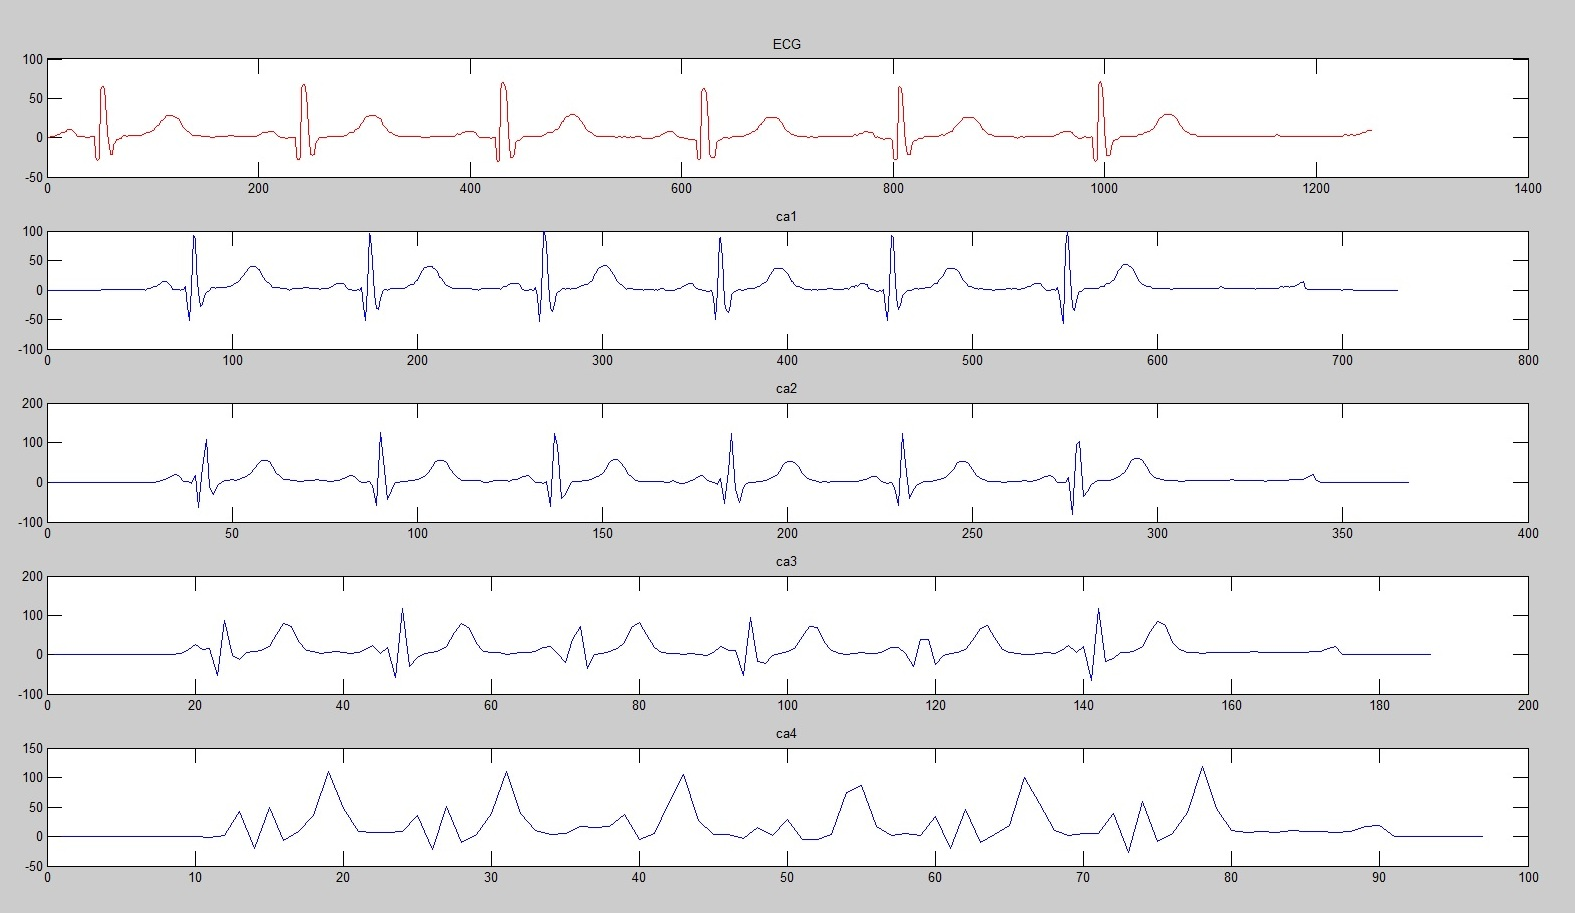
\includegraphics[width=0.5\linewidth] {images/Decomposition.jpg}
  \caption{Low frequencies decomposition}
  \label{fig:decomp}
\end{figure}

At the next stage the obtained time series analyzed visually by operator (user).  Operator chooses the variant that is similar to the original time series.  The chosen variant contains no distortion.  Then the R pikes are determined as maximal values among time moments, where signal amplitude is greater than 60\% of the maximal digital value on the interval.

\begin{figure}[htb]
  \centering
    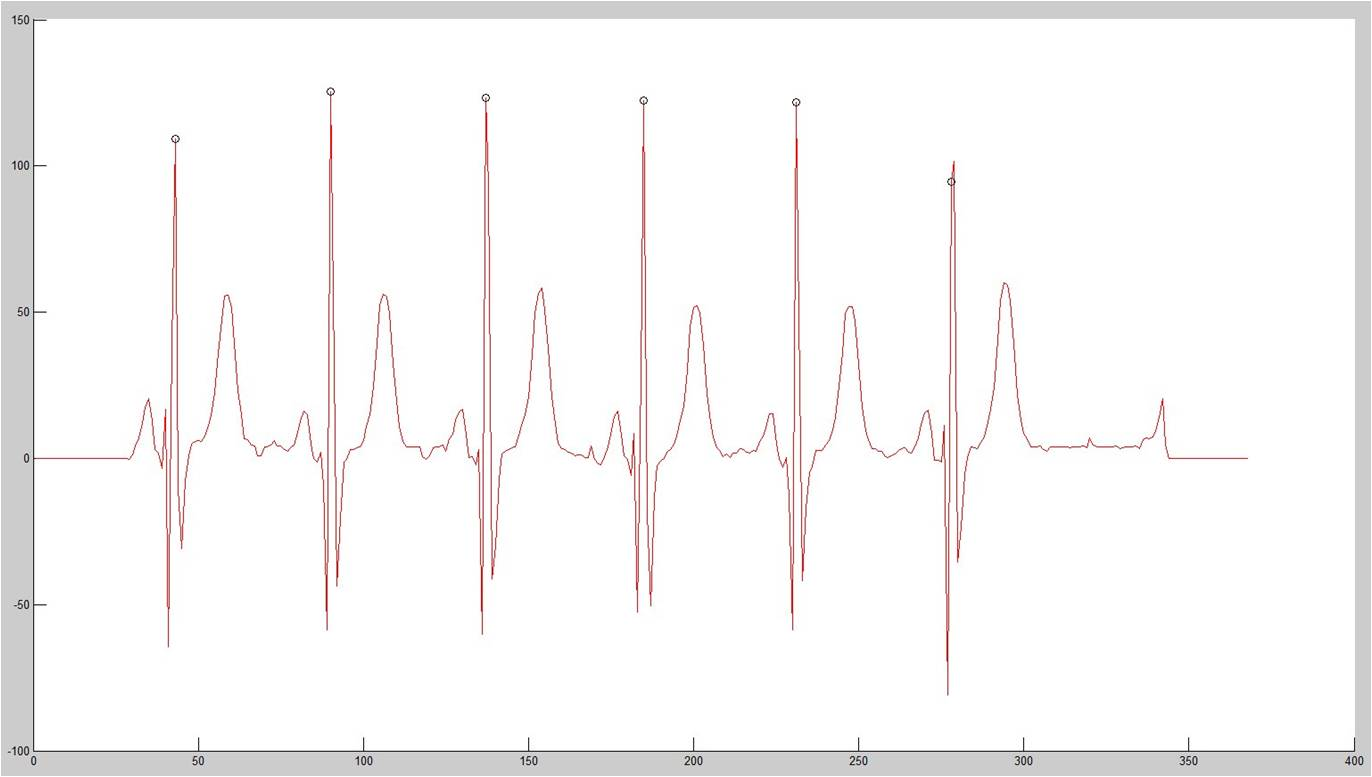
\includegraphics[width=0.5\linewidth] {images/R-pike.jpg}
  \caption{R pike determination}
  \label{fig:determ-R}
\end{figure}
The determined maximal values positions are also filtered according to pike average distance criterion.  The measured pike amplitude is corrected with respect to the basis of the original signal, then the locations of the rest of the pikes are determined (Fig.\ref{fig:fig6} and \ref{fig:fig7}).

\begin{figure}[htb]
  \centering
    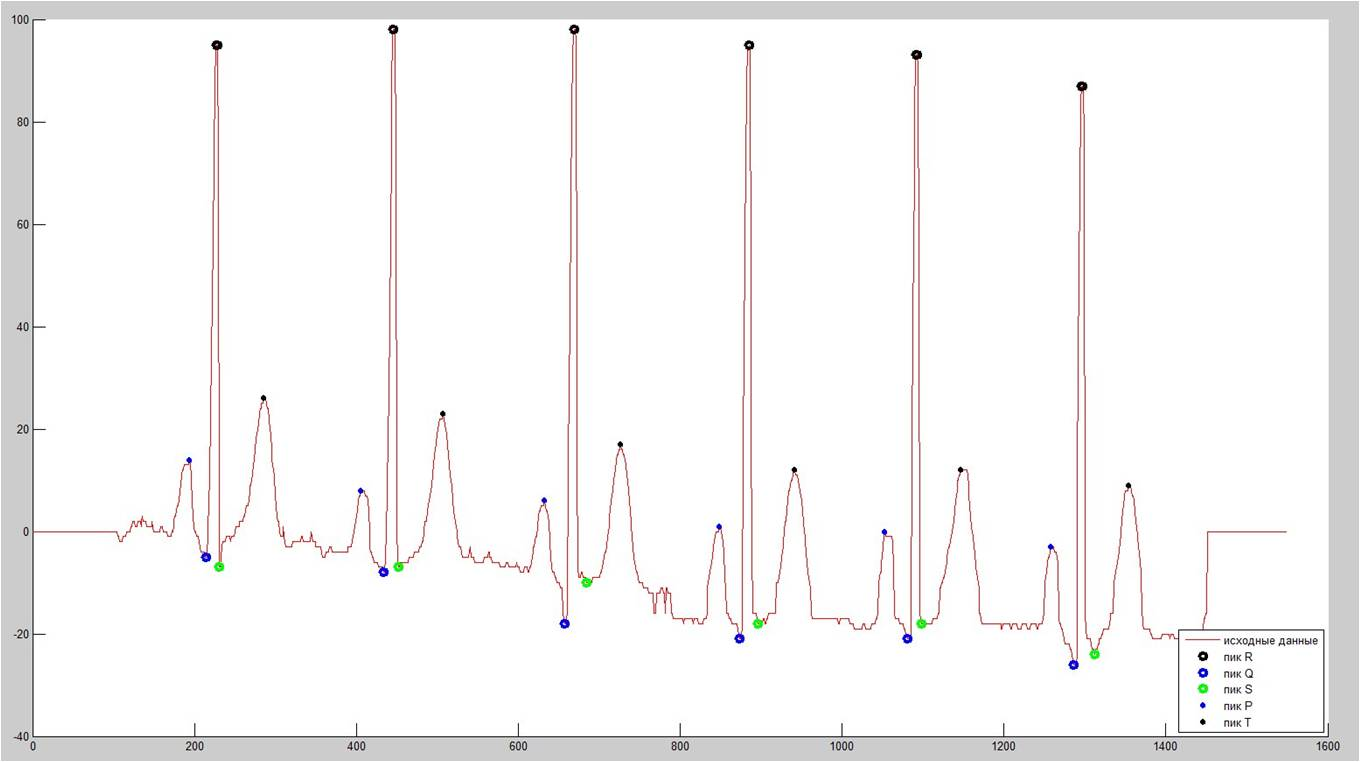
\includegraphics[width=0.5\linewidth] {images/Drift.jpg}
  \caption{R pike determination (base line drift)}
  \label{fig:fig6}
\end{figure}

\begin{figure}[htb]
  \centering
    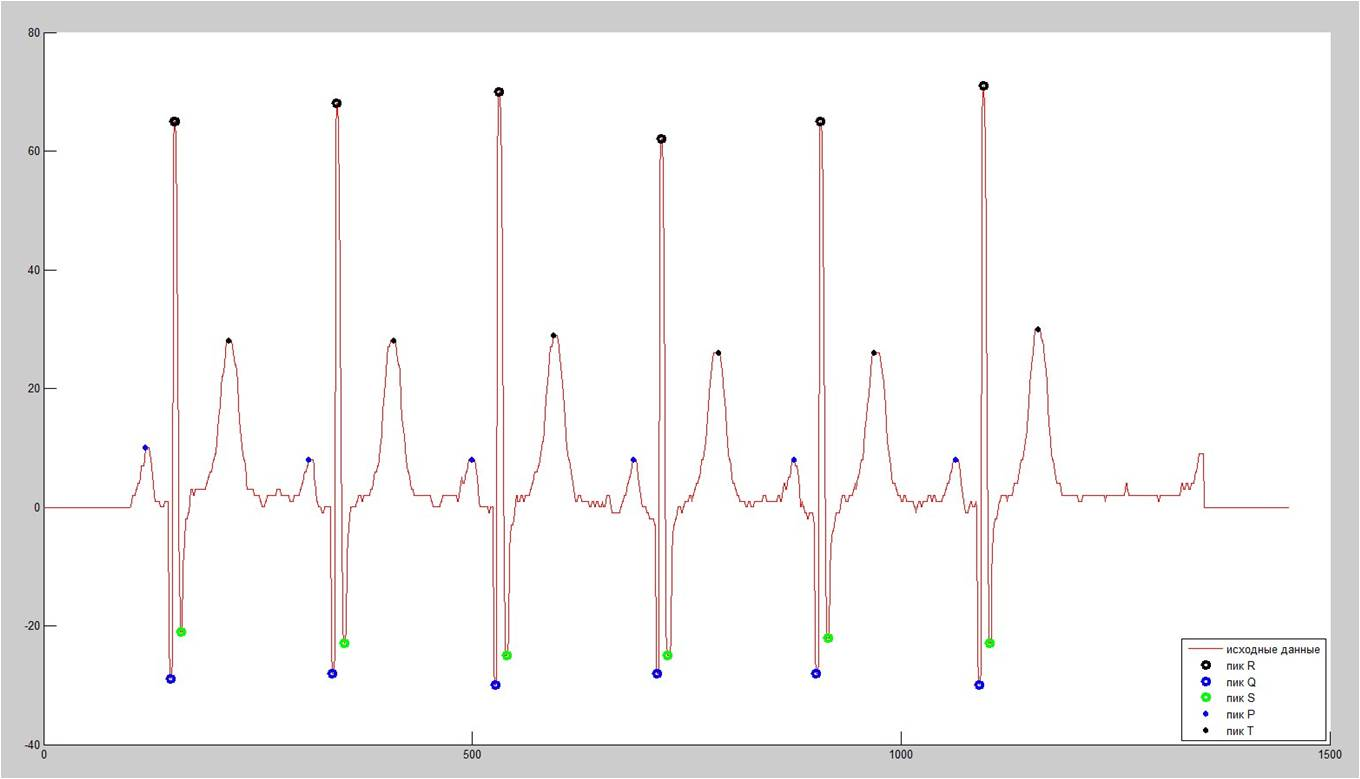
\includegraphics[width=0.5\linewidth] {images/NonDecomposed.jpg}
  \caption{R pike determination (nondecomposed signal)}
  \label{fig:fig7}
\end{figure}

\section{Usage the digitized time series of leads}
\label{sec:applications}

A comparative dynamics analysis of EGC of abnormal hearth rhythms in form of various arrhythmia and conduction disorder has been carried on during patient observations of primary manifestations of undesirable side effects on the months-long anti-tuberculosis chemotherapy.  The abnormalities are as follows (with the number of observations): the rhythm of the right atrium (18 cases), atrioventricular block I st. (7 cases), full blockade of the left His'  leg bundle (2 cases), Brugad syndrome (7 cases), sick sinus syndrome (1 case), pacemaker migration on the atria (2 cases), pacemaker migration on the atria (10 cases), lengthening the interval Q--T (1 case), shortening of P--Q interval --- syndrome premature ventricular heart Сlerk-Levi-Cristesco (CLC) (12 cases), atal syndrome of premature ventricular Wolff-Parkinson-White (WPW), type ``B'' (1 case), acute myocardial infarction with the formation of pathological wave the Q (3 cases), acute myocardial infarction without pike Q (-) but with the rise of segment S-T (3 cases), sinus tachycardia (4 cases), isolated syndrome early ventricular repolarization (4 cases).

\section{Acknowledgment}
\label{sec:acknowledment}

The research is partially supported by Russian Foundation of Basic Research, grant No.~16-07-00554 ``Development of Method for Object Recognition on Raster Images on the Base of Logical Models with Spatial Constraints''.


\section*{Conclusion}
It this paper we briefly described an IT technique for ECG image scans processing and their time series recognition.  The recognition result consists of P, Q, R, S and T section values expressed in qualitative terms, e.g., size, width, and amplitude.  The results will be used as fact data for expert system of structural analysis and interpretation in medical cardiological domains (ES ECG ``SERG'').  We analyzed 156 ECG images obtained by scanning ECG tapes.  The tapes are taken from archives of a hospital, ambulance brigades, and from patients' personal archives.

For some diagrams obtained in an emergency room and in a department of functional diagnostics; a comparative qualitative analysis of ECG time dynamics and accompanying patients supporting documentation has been carried out.  Functionalist now is able to submit the objective values of amplitudes and time intervals of P, Q, R, S and T pikes and the segments of clinically significant QRS complexes in millimeters and milliseconds and in percent relations to a cardiologist.  This resulted in rising the objectivity of dynamics evaluation with the domain criteria and coefficients, mentioned in manuals and guidelines in cardiology, but still rarely used by practitioners due to a lot of mathematical calculation and analysis to be done previously.

Cardiologist carried on an analysis of amplitude dynamics of the amplitudes and the time intervals, and segments parameters, resulting in a safe rational load correction of medicaition dosage for only 2--3 days instead regular 5--6 ones.

The further development of the technique, its software and their implementation in practice to ECG diagnosis expert systems will significantly improve the quality of cardiological monitoring of the patients with a complex comorbid disorders on an interdisciplinary level.

%\bibliographystyle{splncs03}
%\bibliography{example}
 \begin{thebibliography}{99}

 \bibitem{rangaraj} Rangaraj, M.R.: Biomedical Signal Analysis. A Case-Study Approach. IEEE Press and Wiley, New York, NY. (2002). ISBN 0-471-20811-6

 \bibitem{wikipedia} Electrocardiography -- Wikipedia, the free encyclopedia, [Online].  Available:\url{https://en.wikipedia.org/wiki/Electrocardiogram} (current March 2016)

 \bibitem{gonseles} Gonsalez, R.C., Woods, R.E.: Digital Image Processing. MA: Addison-Wesley. (1992)

 \bibitem{1} Gonzalez, R.C., Woods, R.E., Eddins, S.L.: Digital Image Processing Using MATLAB, 2nd ed. Gatesmark Publishing. (2009)

 \bibitem{Ahlstrom-Tomhins} Ahlstrom, M.L., Tomhins, W.J.: Digital filters for real-time ECG signal processing using microprocessors. IEEE Trans. Biomed. Eng. vol.~32. pp.~708--713~(1985)

 \bibitem{Murthy-Rangaraj} Murthy, I.S.N., Rangaraj, M.R.: New concepts for PVC detection. IEEE Trans. Biomed. Eng. vol.~26,~7 pp.~409--416~(1979)

 \bibitem{Pan-Tomhins} Pan, J., Tomhins, W.J.: A real-time QRS detection algorithm. IEEE Trans. Biomed. Eng. vol.~32. pp.~230-236~(1985)

 \bibitem{Daqrouq} Khaled, D., Ibrahim, N.A., Abdel-Rahman, Al-Q.: QRS Complex Detection Based on Symmetry Wavelet Function. In: 5th International MultiConference on Systems, Signals and Devices~(2008)

 \bibitem{Dubrovin} Dubrovin, V.I., Tverdohleb, J.V., Kharchenko, V.V.: R-peaks detection using wavelet Technology. Radioelectronka, informatika, upravlinnya. 2(29)~(2013), [Online].  Available:\url{http://cyberleninka.ru/article/n/r-peaks-detection-using-wavelet-technology} (current~March~2016)

 \bibitem{Gritzali} Gritzali, F., Frangakis, G., Papakonstantinou G.: Detection of the P and T waves in an ECG // Comput. Biomed. Res. vol.~9. pp.~125--132~(1976)


 \end{thebibliography}

%%%%%%%%%%%%%%%%%%%%%%%%%%%%%%%%%%%%%%%%%
%% For the final version of the paper: %%
%%%%%%%%%%%%%%%%%%%%%%%%%%%%%%%%%%%%%%%%%

%% Author information
%\vspace{4ex}\noindent
%\textbf{Author One} is\dots
%
%\bigskip\noindent
%\textbf{Author Two} is\dots
%
%\bigskip\noindent
%\textbf{Author Three} is\dots

%% Reception and acceptance information
%\bigskip
%\paragraph{Received: Month DD, 20YY; Accepted: Month DD, 20YY.}

\end{document}

%%% Local Variables:
%%% mode: latex
%%% TeX-master: t
%%% End:
